\documentclass[10pt]{./acmtrans2e}
\usepackage{hyperref}
\usepackage{amsmath}
\usepackage{amssymb}
\usepackage{amsfonts}
\usepackage{amscd}
\usepackage{amsmath}
\usepackage{latexsym}
\usepackage{graphicx}
\usepackage{geometry}
\usepackage{ifthen}

\hypersetup{
  colorlinks = false,
  urlcolor = blue,
  linkcolor = blue,
  pdfauthor = {Hendrik Speleers},
  pdfkeywords = {Multi-degree splines, MDB-splines, B-splines, Extraction operator},
  pdftitle = {User Manual for the MDB-Spline Toolbox in MATLAB},
  pdfsubject = {MDB-Spline Toolbox},
  pdfpagemode = UseNone
}

\geometry{
  left=4cm,
  right=4cm,
  top=4cm,
  bottom=4cm
}

\newcommand{\Matlab}{\textsc{Matlab} }

\newlength{\tabcont}
\newcommand{\tab}[1]{%
\settowidth{\tabcont}{#1}%
\ifthenelse{\lengthtest{\tabcont < 1cm}}%
{\makebox[1cm][l]{#1}\ignorespaces}%
{\makebox[2cm][l]{#1}\ignorespaces}%
}%

\newcommand{\syntax}[1]{\medskip
\noindent \textbf{Syntax:} \medskip

\texttt{#1}
}

\newenvironment{inputlist}
{\vspace*{0.25cm}
\noindent \textbf{Input parameters:}
\begin{itemize}
}  
{ 
\end{itemize}
}

\newenvironment{outputlist}
{\vspace*{0.075cm}
\noindent \textbf{Output parameters:}
\begin{itemize}
}  
{ 
\end{itemize}
}

\newenvironment{remark}
{\vspace*{0.1cm}
\noindent \textbf{Discussion:} \medskip

}
{
\vspace*{0.2cm}
}

\newenvironment{example}
{\vspace*{0.1cm}
\noindent \textbf{Example:} \vspace*{0.15cm}

\setlength{\parskip}{0.5ex plus 0.5exminus 0.2 ex}
}
{\medskip
}

\newcommand{\paramitem}[2]{\item[] \tab{\texttt{#1}} \tab{: #2} }

\firstfoot{}
\runningfoot{}

\markboth{Hendrik Speleers}{User Manual for the MDS-Spline Toolbox in {MATLAB}}

\title{User Manual for the MDB-Spline Toolbox in {MATLAB}} 

\author{HENDRIK SPELEERS\\University of Rome Tor Vergata}

\begin{document}

\maketitle

\vspace*{-0.7cm}

\section{Introduction}

This guide explains the usage and functionality of the \Matlab toolbox on multi-degree B-splines (MDB-splines) accompanying the article

\begin{center}
\begin{minipage}{0.87\textwidth}
Hendrik Speleers. Algorithm 999: Computation of Multi-Degree B-Splines. \emph{ACM Trans. Math. Softw.} 45, 4, Article 43 (2019), 15 pages.
\end{minipage}
\end{center}

\noindent The toolbox has been developed in \Matlab R2016a but should work with other \Matlab versions as well. 
It can be downloaded from the ACM Collected Algorithms (CALGO). For its installation, just place the toolbox in any directory on your drive, and then add it to the \Matlab path.


\section{Matlab Functions}

The toolbox is divided in two parts: functions dealing with \hyperref[sec:matlab-b]{B-splines} and functions dealing with \hyperref[sec:matlab-mdb]{MDB-splines}. 

\subsection{B-splines}\label{sec:matlab-b}

The main B-spline data-structure is called \emph{B-spline patch} and identifies a certain B-spline space. It contains the open knot vector, spline degree, and spline dimension.
Note that it would be sufficient to store only the knot vector; however, the other parameters simplify further operations.

The following \Matlab functions are provided for working with B-spline patches.
\begin{itemize}
  \item[$\bullet$] \hyperref[sec:matlab-b-patch]{\texttt{B\_patch}}: 
     construction of a B-spline patch with open knot vector;
  \item[$\bullet$] \hyperref[sec:matlab-b-domain]{\texttt{B\_domain}}: 
     computation of the end points of the domain related to a patch;
  \item[$\bullet$] \hyperref[sec:matlab-b-greville]{\texttt{B\_greville}}: 
     computation of the Greville points;
  \item[$\bullet$] \hyperref[sec:matlab-b-evaluation-all]{\texttt{B\_evaluation\_all}}: 
     evaluation of all B-splines in given points;
  \item[$\bullet$] \hyperref[sec:matlab-b-evaluation-spline]{\texttt{B\_evaluation\_spline}}: 
     evaluation of a spline in given points;
  \item[$\bullet$] \hyperref[sec:matlab-b-diffend-all]{\texttt{B\_diffend\_all}}: 
     full differentiation of all B-splines at one end point up to a given order;
  \item[$\bullet$] \hyperref[sec:matlab-b-differentiation-all]{\texttt{B\_differentiation\_all}}: 
     differentiation of all B-splines in given points;
  \item[$\bullet$] \hyperref[sec:matlab-b-differentiation-spline]{\texttt{B\_differentiation\_spline}}: 
     differentiation of a spline in given points;
  \item[$\bullet$] \hyperref[sec:matlab-b-visualization-all]{\texttt{B\_visualization\_all}}: 
     visualization of all B-splines;
  \item[$\bullet$] \hyperref[sec:matlab-b-visualization-spline]{\texttt{B\_visualization\_spline}}: 
     visualization of a spline;
  \item[$\bullet$] \hyperref[sec:matlab-b-conversion]{\texttt{B\_conversion}}: 
     conversion from source to destination B-spline form.
\end{itemize}

%------------------------------------------------------------------

\subsubsection{B\_patch} \label{sec:matlab-b-patch}

This function prepares the data-structure for a B-spline patch, starting from a sequence of polynomial segments of fixed degree and smoothness relations. The B-spline patch is a structure array containing the open knot vector \texttt{U}, spline degree \texttt{p}, and spline dimension~\texttt{n}. 

\pagebreak
\syntax{P = B\_patch(p, xx, kk)}

\begin{inputlist}
  \paramitem{p}{B-spline degree}
  \paramitem{xx}{vector of break points}
  \paramitem{kk}{smoothness vector (optional)}
\end{inputlist}

\begin{outputlist}
  \paramitem{P}{B-spline patch}
\end{outputlist}

\begin{remark}
\noindent The parameter \texttt{p} is a non-negative integer scalar, the parameter \texttt{xx} is a vector consisting of a strictly increasing sequence of real values (indicating the different segments), and the parameter \texttt{kk} can be a scalar or a vector whose elements are non-negative integers less than the value of \texttt{p}.
If \texttt{kk} is a scalar, smoothness \texttt{kk} is imposed at the break point \texttt{xx(i+1)}, and
if \texttt{kk} is a vector, smoothness \texttt{kk(i)} is imposed at the break point \texttt{xx(i+1)},
for \texttt{i = 1:length(xx)-2}.
Hence, \texttt{length(kk)} should be equal to \texttt{1} or \texttt{length(xx)-2}. 
When no smoothness is specified, \texttt{kk = 0} is assumed.
\end{remark}

\begin{example}
\noindent Create a B-spline patch of degree $4$ and smoothness $C^2$ defined on a domain partitioned in the two intervals $[0, 3]$ and $[3, 4]$: 
\medskip

\texttt{>> P = B\_patch(4, [0, 3, 4], 2)}

\texttt{P = }

\texttt{\ \ \ \ p:\ 4}

\texttt{\ \ \ \ n:\ 7}

\texttt{\ \ \ \ U:\ [0 0 0 0 0 3 3 4 4 4 4 4]}
\end{example}

%------------------------------------------------------------------

\subsubsection{B\_domain} \label{sec:matlab-b-domain}

This function computes the end points of the domain specified by a given B-spline patch. 

\syntax{[a, b] = B\_domain(P)}

\begin{inputlist}
  \paramitem{P}{B-spline patch}
\end{inputlist}

\begin{outputlist}
  \paramitem{a}{left end point}
  \paramitem{b}{right end point}
\end{outputlist}

\vspace*{-0.45cm}
\begin{example}
\noindent Create a B-spline patch and show the end points of its domain:
\medskip

\texttt{>> P = B\_patch(4, [0, 3, 4], 2);}

\texttt{>> [a, b] = B\_domain(P)}

\texttt{a =}

\texttt{\ \ \ \ \ 0}

\texttt{b =}

\texttt{\ \ \ \ \ 4}
\end{example}

%------------------------------------------------------------------

\subsubsection{B\_greville} \label{sec:matlab-b-greville}

This function computes the Greville points of a given B-spline patch, i.e., the coefficients of the B-spline form of the identity function.

\syntax{gg = B\_greville(P)}

\begin{inputlist}
  \paramitem{P}{B-spline patch}
\end{inputlist}

\begin{outputlist}
  \paramitem{gg}{vector of Greville points}
\end{outputlist}

\begin{remark}
\noindent 
Each element of the vector \texttt{gg} corresponds to a B-spline, so \texttt{length(gg)} equals \texttt{P.n}.
\end{remark}

\begin{example}
\noindent Create a B-spline patch and show its Greville points:
\medskip

\texttt{>> P = B\_patch(4, [0, 3, 4], 2);}

\texttt{>> gg = B\_greville(P)}

\texttt{gg =}

\texttt{\ \ \ \ \ \ \ \ \ 0\ \ \ \ 0.7500\ \ \ \ 1.5000\ \ \ \ 2.5000\ \ \ \ 3.5000\ \ \ \ 3.7500\ \ \ \ 4.0000}
\end{example}

%------------------------------------------------------------------

\subsubsection{B\_evaluation\_all} \label{sec:matlab-b-evaluation-all}

This function evaluates all B-splines of a B-spline patch at a given set of points, and stores the corresponding values in a matrix.

\syntax{M = B\_evaluation\_all(P, xx, cl)}

\begin{inputlist}
  \paramitem{P}{B-spline patch}
  \paramitem{xx}{vector of evaluation points}
  \paramitem{cl}{closed domain if true (optional)}
\end{inputlist}

\pagebreak
\vspace*{-0.4cm}
\begin{outputlist}
  \paramitem{M}{evaluation matrix}
\end{outputlist}

\begin{remark}
\noindent The parameter \texttt{cl} takes a boolean value.
If \texttt{cl} is \texttt{false}, then the B-spline values are computed by the B-spline recurrence relation on the half-open domain of the patch and are zero outside; otherwise, at the right end point, they are computed by taking limits from the left (making the spline space symmetric on the closed domain).
When no value is specified, \texttt{cl = true} is assumed.
Each row in the resulting matrix \texttt{M} corresponds to a B-spline and each column to an evaluation point, so \texttt{size(M)} equals \texttt{[P.n, length(xx)]}.~
\end{remark}

\begin{example}
\noindent Create a B-spline patch and evaluate all the corresponding B-splines at the break points of the patch:
\medskip

\texttt{>> P = B\_patch(4, [0, 3, 4], 2);}

\texttt{>> M = B\_evaluation\_all(P, [0, 3, 4])}

\texttt{M =}

\texttt{\ \ \ \ 1.0000\ \ \ \ \ \ \ \ \ 0\ \ \ \ \ \ \ \ \ 0}

\texttt{\ \ \ \ \ \ \ \ \ 0\ \ \ \ \ \ \ \ \ 0\ \ \ \ \ \ \ \ \ 0}

\texttt{\ \ \ \ \ \ \ \ \ 0\ \ \ \ 0.0625\ \ \ \ \ \ \ \ \ 0}

\texttt{\ \ \ \ \ \ \ \ \ 0\ \ \ \ 0.3750\ \ \ \ \ \ \ \ \ 0}

\texttt{\ \ \ \ \ \ \ \ \ 0\ \ \ \ 0.5625\ \ \ \ \ \ \ \ \ 0}

\texttt{\ \ \ \ \ \ \ \ \ 0\ \ \ \ \ \ \ \ \ 0\ \ \ \ \ \ \ \ \ 0}

\texttt{\ \ \ \ \ \ \ \ \ 0\ \ \ \ \ \ \ \ \ 0\ \ \ \ 1.0000}
\end{example}

%------------------------------------------------------------------

\subsubsection{B\_evaluation\_spline} \label{sec:matlab-b-evaluation-spline}

This function evaluates a spline in B-spline form at a given set of points, and stores the corresponding values in a vector.

\syntax{ss = B\_evaluation\_spline(P, cc, xx)}

\begin{inputlist}
  \paramitem{P}{B-spline patch}
  \paramitem{cc}{vector of coefficients}
  \paramitem{xx}{vector of evaluation points}
\end{inputlist}

\begin{outputlist}
  \paramitem{ss}{vector of spline evaluation values}
\end{outputlist}

\pagebreak
\vspace*{-0.4cm}
\begin{remark}
\noindent Each element of the vector \texttt{cc} corresponds to a B-spline in the B-spline patch. Hence, \texttt{length(cc)} should be equal to \texttt{P.n}. Each element of the resulting vector \texttt{ss} corresponds to an evaluation point, so \texttt{length(ss)} equals \texttt{length(xx)}.
\end{remark}

\begin{example}
\noindent Create a B-spline patch and a vector of coefficients, and then evaluate the corresponding spline in B-spline form at the break points of the patch:
\medskip

\texttt{>> P = B\_patch(4, [0, 3, 4], 2);}

\texttt{>> cc = [1, 2, 3, 4, 4, 3, 2];}

\texttt{>> ss = B\_evaluation\_spline(P, cc, [0, 3, 4])}

\texttt{ss =}

\texttt{\ \ \ \ 1.0000\ \ \ \ 3.9375\ \ \ \ 2.0000}

\end{example}

%------------------------------------------------------------------

\subsubsection{B\_diffend\_all} \label{sec:matlab-b-diffend-all}

This function evaluates all the derivatives, up to a certain order $r$, of all B-splines of a B-spline patch at one of the two end points of the domain, and stores the corresponding values in a matrix.

\syntax{K = B\_diffend\_all(P, r, el)}

\begin{inputlist}
  \paramitem{P}{B-spline patch}
  \paramitem{r}{maximum order of derivative}
  \paramitem{el}{left end if true, right end otherwise (optional)}
\end{inputlist}

\begin{outputlist}
  \paramitem{K}{differentiation matrix at end point up to \texttt{r}-th order}
\end{outputlist}

\begin{remark}
\noindent The parameter \texttt{r} is a non-negative integer.
The parameter \texttt{el} takes a boolean value. If \texttt{el} is \texttt{true}, then the left end point of the domain is selected; otherwise, the right end point. When no value is specified, \texttt{el = true} is assumed.
Each row in the resulting matrix \texttt{K} corresponds to a B-spline and each column to a derivative, so \texttt{size(K)} equals \texttt{[P.n, r+1]}.
\end{remark}

\begin{example}
\noindent Create a B-spline patch and evaluate all derivatives, up to fourth order, of all the corresponding B-splines at the right end point of the domain:
\medskip

\texttt{>> P = B\_patch(4, [0, 3, 4], 2);}

\texttt{>> K = B\_diffend\_all(P, 4, false)}

\pagebreak

\texttt{K =}

\texttt{\ \ \ \ \ \ \ \ \ 0\ \ \ \ \ \ \ \ \ 0\ \ \ \ \ \ \ \ \ 0\ \ \ \ \ \ \ \ \ 0\ \ \ \ \ \ \ \ \ 0}

\texttt{\ \ \ \ \ \ \ \ \ 0\ \ \ \ \ \ \ \ \ 0\ \ \ \ \ \ \ \ \ 0\ \ \ \ \ \ \ \ \ 0\ \ \ \ \ \ \ \ \ 0}

\texttt{\ \ \ \ \ \ \ \ \ 0\ \ \ \ \ \ \ \ \ 0\ \ \ \ \ \ \ \ \ 0\ \ \ \ \ \ \ \ \ 0\ \ \ \ 1.5000}

\texttt{\ \ \ \ \ \ \ \ \ 0\ \ \ \ \ \ \ \ \ 0\ \ \ \ \ \ \ \ \ 0\ \ \ -6.0000\ \ -15.0000}

\texttt{\ \ \ \ \ \ \ \ \ 0\ \ \ \ \ \ \ \ \ 0\ \ \ 12.0000\ \ \ 54.0000\ \ \ 85.5000}

\texttt{\ \ \ \ \ \ \ \ \ 0\ \ \ -4.0000\ \ -24.0000\ \ -72.0000\ \ -96.0000}

\texttt{\ \ \ \ 1.0000\ \ \ \ 4.0000\ \ \ 12.0000\ \ \ 24.0000\ \ \ 24.0000}
\end{example}

%------------------------------------------------------------------

\subsubsection{B\_differentiation\_all} \label{sec:matlab-b-differentiation-all}

This function evaluates the $r$-th order derivative of all B-splines of a B-spline patch at a given set of points, and stores the corresponding values in a matrix.

\syntax{M = B\_differentiation\_all(P, r, xx, cl)}

\begin{inputlist}
  \paramitem{P}{B-spline patch}
  \paramitem{r}{order of derivative}
  \paramitem{xx}{vector of evaluation points}
  \paramitem{cl}{closed domain if true (optional)}
\end{inputlist}

\begin{outputlist}
  \paramitem{M}{differentiation matrix}
\end{outputlist}

\begin{remark}
\noindent The parameter \texttt{r} is a non-negative integer.
The parameter \texttt{cl} takes a boolean value.
If \texttt{cl} is \texttt{false}, then the B-spline values are computed by the B-spline recurrence relation on the half-open domain of the patch and are zero outside; otherwise, at the right end point, they are computed by taking limits from the left (making the spline space symmetric on the closed domain).
When no value is specified, \texttt{cl = true} is assumed.
Each row in the resulting matrix \texttt{M} corresponds to a B-spline and each column to an evaluation point, so \texttt{size(M)} equals \texttt{[P.n, length(xx)]}.
\end{remark}

\begin{example}
\noindent Create a B-spline patch and evaluate the first derivative of all the corresponding B-splines at the break points of the patch:
\medskip

\texttt{>> P = B\_patch(4, [0, 3, 4], 2);}

\texttt{>> M = B\_differentiation\_all(P, 1, [0, 3, 4])}

\pagebreak 

\texttt{M =}

\texttt{\ \ \ -1.3333\ \ \ \ \ \ \ \ \ 0\ \ \ \ \ \ \ \ \ 0}

\texttt{\ \ \ \ 1.3333\ \ \ \ \ \ \ \ \ 0\ \ \ \ \ \ \ \ \ 0}

\texttt{\ \ \ \ \ \ \ \ \ 0\ \ \ -0.2500\ \ \ \ \ \ \ \ \ 0}

\texttt{\ \ \ \ \ \ \ \ \ 0\ \ \ -0.5000\ \ \ \ \ \ \ \ \ 0}

\texttt{\ \ \ \ \ \ \ \ \ 0\ \ \ \ 0.7500\ \ \ \ \ \ \ \ \ 0}

\texttt{\ \ \ \ \ \ \ \ \ 0\ \ \ \ \ \ \ \ \ 0\ \ \ -4.0000}

\texttt{\ \ \ \ \ \ \ \ \ 0\ \ \ \ \ \ \ \ \ 0\ \ \ \ 4.0000}
\end{example}

%------------------------------------------------------------------

\subsubsection{B\_differentiation\_spline} \label{sec:matlab-b-differentiation-spline}

This function evaluates the $r$-th order derivative of a spline in B-spline form at a given set of points, and stores the corresponding values in a vector.

\syntax{ss = B\_differentiation\_spline(P, r, cc, xx)}

\begin{inputlist}
  \paramitem{P}{B-spline patch}
  \paramitem{r}{order of derivative}
  \paramitem{cc}{vector of coefficients}
  \paramitem{xx}{vector of evaluation points}
\end{inputlist}

\begin{outputlist}
  \paramitem{ss}{vector of \texttt{r}-th order derivative spline values}
\end{outputlist}

\begin{remark}
\noindent The parameter \texttt{r} is a non-negative integer.
Each element of the vector \texttt{cc} corresponds to a B-spline in the B-spline patch. Hence, \texttt{length(cc)} should be equal to \texttt{P.n}. Each element of the resulting vector \texttt{ss} corresponds to an evaluation point, so \texttt{length(ss)} equals \texttt{length(xx)}.
\end{remark}

\begin{example}
\noindent Create a B-spline patch and a vector of coefficients, and then evaluate the first derivative of the corresponding spline in B-spline form at the break points of the patch:
\medskip

\texttt{>> P = B\_patch(4, [0, 3, 4], 2);}

\texttt{>> cc = [1, 2, 3, 4, 4, 3, 2];}

\texttt{>> ss = B\_differentiation\_spline(P, 1, cc, [0, 3, 4])}

\texttt{ss =}

\texttt{\ \ \ \ 1.3333\ \ \ \ 0.2500\ \ \ -4.0000}

\end{example}

%------------------------------------------------------------------

\subsubsection{B\_visualization\_all} \label{sec:matlab-b-visualization-all}

This function visualizes all B-splines of a B-spline patch.

\syntax{B\_visualization\_all(P, n, specs)}

\begin{inputlist}
  \paramitem{P}{B-spline patch}
  \paramitem{n}{number of evaluation points (optional)}
  \paramitem{specs}{pass any number of plot specifications (optional)}
\end{inputlist}

\begin{remark}
\noindent The parameter \texttt{n} is a positive integer. When no value is specified, \texttt{n = 100} is assumed.
The parameter \texttt{specs} allows for any number of input arguments, which are passed on to the function \texttt{plot}. We refer the reader to the documentation of \texttt{plot} for all the plotting options.
\end{remark}

\begin{example}
\noindent Create a B-spline patch and plot all the corresponding B-splines:
\medskip

\texttt{>> P = B\_patch(4, [0, 3, 4], 2);}

\texttt{>> B\_visualization\_all(P, 100, 'LineWidth', 2);}

\begin{center}
  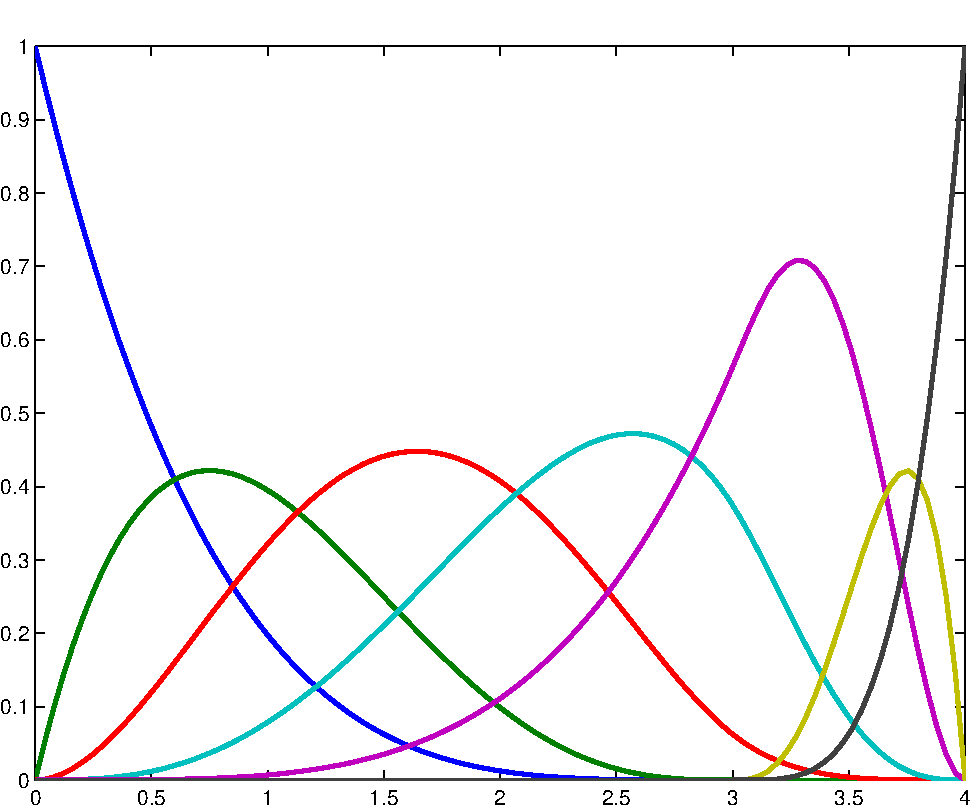
\includegraphics[width=4.5cm]{manual_ex_bspline0}
\end{center}
\vspace*{-0.35cm}
\end{example}

%------------------------------------------------------------------

\subsubsection{B\_visualization\_spline} \label{sec:matlab-b-visualization-spline}

This function visualizes a spline in B-spline form.

\syntax{B\_visualization\_spline(P, cc, n, specs)}

\begin{inputlist}
  \paramitem{P}{B-spline patch}
  \paramitem{cc}{vector of coefficients}
  \paramitem{n}{number of evaluation points (optional)}
  \paramitem{specs}{pass any number of plot specifications (optional)}
\end{inputlist}

\vspace*{-0.4cm}
\begin{remark}
\noindent Each element of the vector \texttt{cc} corresponds to a B-spline in the B-spline patch. Hence, \texttt{length(cc)} should be equal to \texttt{P.n}.
The parameter \texttt{n} is a positive integer. When no value is specified, \texttt{n = 100} is assumed.
The parameter \texttt{specs} allows for any number of input arguments, which are passed on to the function \texttt{plot}. We refer the reader to the documentation of \texttt{plot} for all the plotting options.
\end{remark}

\begin{example}
\noindent Create a B-spline patch and a vector of coefficients, and then plot the corresponding spline in B-spline form:
\medskip

\texttt{>> P = B\_patch(4, [0, 3, 4], 2);}

\texttt{>> cc = [1, 2, 3, 4, 4, 3, 2];}

\texttt{>> B\_visualization\_spline(P, cc, 100, 'LineWidth', 2);}

\begin{center}
  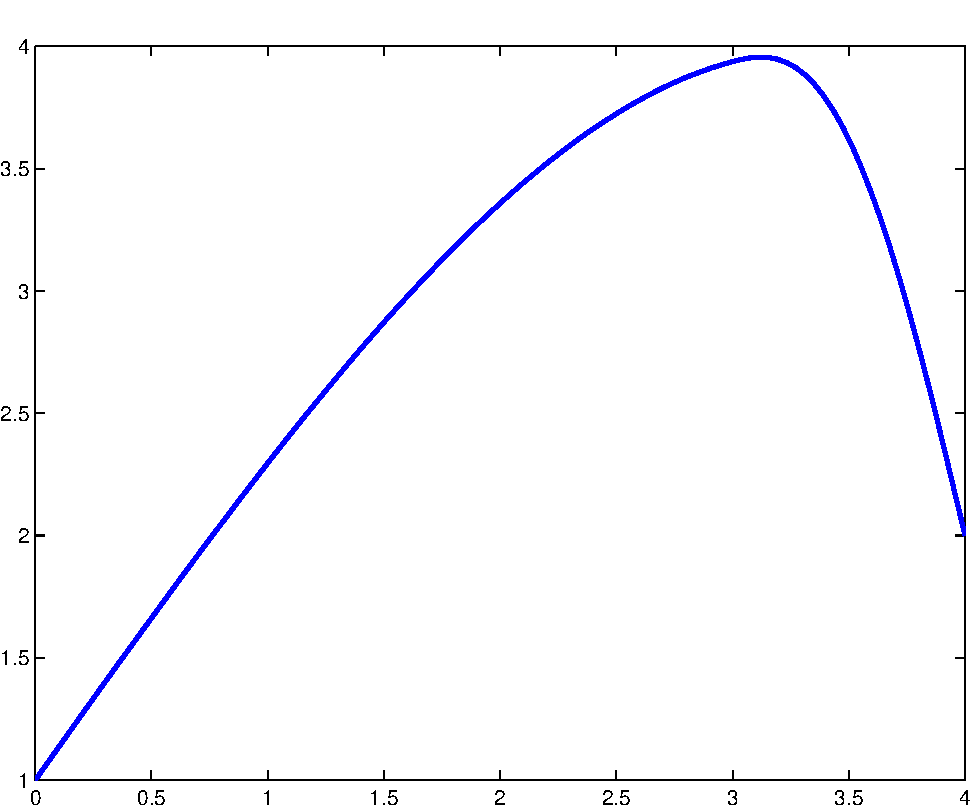
\includegraphics[width=4.5cm]{manual_ex_bspline1}
\end{center}
\vspace*{-0.35cm}
\end{example}

%------------------------------------------------------------------

\subsubsection{B\_conversion} \label{sec:matlab-b-conversion}

This function converts a spline in B-spline form into another B-spline form.
The conversion is exact when the source and destination B-spline patches imply nested spaces.

\syntax{ccd = B\_conversion(Pd, Ps, ccs)}

\begin{inputlist}
  \paramitem{Pd}{destination B-spline patch}
  \paramitem{Ps}{source B-spline patch}
  \paramitem{ccs}{source coefficient vector}
\end{inputlist}

\begin{outputlist}
  \paramitem{ccd}{destination coefficient vector}
\end{outputlist}

\begin{remark}
\noindent The B-spline patches \texttt{Ps} and \texttt{Pd} preferably share the same break points for the best conversion results.
Each element of the vector \texttt{ccs} corresponds to a B-spline in the B-spline patch \texttt{Ps}. Hence, \texttt{length(ccs)} should be equal to \texttt{Ps.n}. Similarly, each element of the resulting vector \texttt{ccd} corresponds to a B-spline in the B-spline patch \texttt{Pd}.
\end{remark}

\begin{example}
\noindent Create a B-spline patch of degree $4$ and a vector of coefficients; then, raise the degree to~$7$ and compute the coefficients of the new B-spline form:
\medskip

\texttt{>> Ps = B\_patch(4, [0, 3, 4], 2);}

\texttt{>> ccs = [1, 2, 3, 4, 4, 3, 2];}

\texttt{>> Pd = B\_patch(7, [0, 3, 4], 2);}

\texttt{>> ccd = B\_conversion(Pd, Ps, ccs)}

\texttt{ccd =}

\texttt{\ \ Columns 1 through 7}

\texttt{\ \ \ \ 1.0000\ \ \ \ 1.5714\ \ \ \ 2.1429\ \ \ \ 2.6857\ \ \ \ 3.1696\ \ \ \ 3.5625\ \ \ \ 3.9196}

\texttt{\ \ Columns 8 through 13}

\texttt{\ \ \ \ 3.9911\ \ \ \ 3.8839\ \ \ \ 3.6000\ \ \ \ 3.1429\ \ \ \ 2.5714\ \ \ \ 2.0000}
\end{example}

%------------------------------------------------------------------

\subsection{MDB-splines}\label{sec:matlab-mdb}

The main MDB-spline data-structure is called \emph{MDB-spline multi-patch}. It contains a vector of B-spline patches and the corresponding cumulative dimension. 

The following \Matlab functions are provided for core operations on MDB-spline multi-patches.
\begin{itemize}
  \item[$\bullet$] \hyperref[sec:matlab-mdb-patch]{\texttt{MDB\_patch}}: 
     construction of an MDB-spline multi-patch from B-spline segments;
  \item[$\bullet$] \hyperref[sec:matlab-mdb-patch-poly]{\texttt{MDB\_patch\_poly}}: 
    construction of an MDB-spline multi-patch from polynomial segments; 
  \item[$\bullet$] \hyperref[sec:matlab-mdb-extraction]{\texttt{MDB\_extraction}}: 
    computation of the multi-degree spline extraction matrix;
  \item[$\bullet$] \hyperref[sec:matlab-mdb-extraction-periodic]{\texttt{MDB\_extraction\_periodic}}: 
    computation of the multi-degree spline extraction matrix with periodicity;
  \item[$\bullet$] \hyperref[sec:matlab-mdb-nullspace]{\texttt{MDB\_nullspace}}: 
    computation of the left null-space of a column of matrix \texttt{L} in the extraction procedure;
    this is an auxiliary function for the functions \texttt{MDB\_extraction} and \texttt{MDB\_extraction\_periodic}, and has no stand-alone usage;
  \item[$\bullet$] \hyperref[sec:matlab-mdb-extraction-local]{\texttt{MDB\_extraction\_local}}: 
    computation of the local multi-degree spline extraction matrix corresponding to a single patch;
\end{itemize}
Furthermore, the following \Matlab functions are provided for working with MDB-splines. Thanks to the multi-degree spline extraction operator, their implementation can be easily redirected to their B-spline analogues described in Section~\ref{sec:matlab-b}.
\begin{itemize}
  \item[$\bullet$] \hyperref[sec:matlab-mdb-domain]{\texttt{MDB\_domain}}: 
    computation of the end points of the domain related to a multi-patch;
  \item[$\bullet$] \hyperref[sec:matlab-mdb-greville]{\texttt{MDB\_greville}}: 
    computation of the multi-degree Greville points;
  \item[$\bullet$] \hyperref[sec:matlab-mdb-evaluation-all]{\texttt{MDB\_evaluation\_all}}: 
    evaluation of all MDB-splines in given points;
  \item[$\bullet$] \hyperref[sec:matlab-mdb-evaluation-spline]{\texttt{MDB\_evaluation\_spline}}: 
    evaluation of a multi-degree spline in given points;
  \item[$\bullet$] \hyperref[sec:matlab-mdb-differentiation-all]{\texttt{MDB\_differentiation\_all}}: 
    differentiation of all MDB-splines in given points;
  \item[$\bullet$] \hyperref[sec:matlab-mdb-differentiation-spline]{\texttt{MDB\_differentiation\_spline}}: 
    differentiation of a multi-degree spline in given points;
  \item[$\bullet$] \hyperref[sec:matlab-mdb-visualization-all]{\texttt{MDB\_visualization\_all}}: 
    visualization of all MDB-splines;
  \item[$\bullet$] \hyperref[sec:matlab-mdb-visualization-spline]{\texttt{MDB\_visualization\_spline}}: 
    visualization of a multi-degree spline;
  \item[$\bullet$] \hyperref[sec:matlab-mdb-conversion]{\texttt{MDB\_conversion}}: 
    conversion from source to destination MDB-spline form.
\end{itemize}

%------------------------------------------------------------------

\subsubsection{MDB\_patch} \label{sec:matlab-mdb-patch}

This function prepares the data-structure for an MDB-spline multi-patch, starting from a sequence of B-spline segments. The MDB-spline multi-patch is a structure array containing a vector of B-spline patches \texttt{P} and the corresponding cumulative dimension \texttt{mu}. 

\syntax{MP = MDB\_patch(PP)}

\begin{inputlist}
  \paramitem{PP}{vector of B-spline patches}
\end{inputlist}

\begin{outputlist}
  \paramitem{MP}{MDB-spline multi-patch}
\end{outputlist}

\begin{example}
\noindent Create an MDB-spline multi-patch consisting of two B-spline patches with different degrees ($3$ and $4$) but with the same smoothness $C^2$: 
\medskip

\texttt{>> P1 = B\_patch(3, [0, 1, 3], 2);}

\texttt{>> P2 = B\_patch(4, [3, 4, 6], 2);}

\texttt{>> MP = MDB\_patch([P1, P2])}

\texttt{MP = }

\texttt{\ \ \ \ \ P:\ [1x2 struct]}

\texttt{\ \ \ \ mu:\ [0 5 12]}

\texttt{>> MP.P(1)}

\texttt{ans =}

\texttt{\ \ \ \ p:\ 3}

\texttt{\ \ \ \ n:\ 5}

\texttt{\ \ \ \ U:\ [0 0 0 0 1 3 3 3 3]}

\texttt{>> MP.P(2)}

\texttt{ans =}

\texttt{\ \ \ \ p:\ 4}

\texttt{\ \ \ \ n:\ 7}

\texttt{\ \ \ \ U:\ [3 3 3 3 3 4 4 6 6 6 6 6]}    
\end{example}

%------------------------------------------------------------------

\subsubsection{MDB\_patch\_poly} \label{sec:matlab-mdb-patch-poly}

This function prepares the data-structure for an MDB-spline multi-patch, starting from a sequence of polynomial segments and smoothness relations.
The MDB-spline multi-patch is a structure array containing a vector of B-spline patches \texttt{P} and the corresponding cumulative dimension \texttt{mu}. Consecutive polynomial segments of the same degree are merged into a single B-spline patch (unless specified otherwise).

\syntax{[MP, rr] = MDB\_patch\_poly(pp, xx, kk, mg)}

\begin{inputlist}
  \paramitem{pp}{vector of polynomial degrees}
  \paramitem{xx}{vector of break points}
  \paramitem{kk}{smoothness vector (optional)}
  \paramitem{mg}{same degree merged if true (optional)}
\end{inputlist}

\begin{outputlist}
  \paramitem{MP}{MDB-spline multi-patch}
  \paramitem{rr}{MDB-spline smoothness vector (optional)}
\end{outputlist}

\begin{remark}
\noindent The parameter \texttt{pp} is a vector consisting of non-negative integer values, and the parameter \texttt{xx} is a vector consisting of a strictly increasing sequence of real values (indicating the different segments), such that
\texttt{length(pp)} equals \texttt{length(xx)-1}. 
The parameter \texttt{kk} can be a scalar or a vector whose elements are non-negative integers.
If \texttt{kk} is a scalar, then \texttt{kk} should be less than \texttt{min(pp)}, and smoothness \texttt{kk} is imposed at the break point \texttt{xx(i+1)} for \texttt{i = 1:length(xx)-2}.
On the other hand, if \texttt{kk} is a vector, then \texttt{kk(i)} should be less than \texttt{min(pp(i),pp(i+1))}, and smoothness \texttt{kk(i)} is imposed at the break point \texttt{xx(i+1)} for \texttt{i = 1:length(xx)-2}.
Hence, \texttt{length(kk)} should be equal to \texttt{1} or \texttt{length(xx)-2}. 
When no smoothness is specified, \texttt{kk = 0} is assumed. 
The parameter \texttt{mg} takes a boolean value.
If \texttt{mg} is \texttt{true}, then consecutive polynomial segments of the same degree are merged into a single B-spline patch; otherwise, they are not merged. When no value is specified, \texttt{mg = true} is assumed.
The resulting vector \texttt{rr} represents the corresponding smoothness between the B-spline patches, so 
\texttt{length(rr)} equals \texttt{length(MP.P)-1}.
\end{remark}

\begin{example}
\noindent Create an MDB-spline multi-patch consisting of four polynomial segments with different degrees ($3$ and $4$) that are connected with smoothness $C^2$: 
\medskip

\texttt{>> [MP, rr] = MDB\_patch\_poly([3, 3, 4, 4], [0, 1, 3, 4, 6], 2)}

\texttt{MP = }

\texttt{\ \ \ \ \ P:\ [1x2 struct]}

\texttt{\ \ \ \ mu:\ [0 5 12]}

\texttt{rr = }

\texttt{\ \ \ \ \ 2}

\texttt{>> MP.P(1)}

\texttt{ans =}

\texttt{\ \ \ \ p:\ 3}

\texttt{\ \ \ \ n:\ 5}

\texttt{\ \ \ \ U:\ [0 0 0 0 1 3 3 3 3]}

\texttt{>> MP.P(2)}

\texttt{ans =}

\texttt{\ \ \ \ p:\ 4}

\texttt{\ \ \ \ n:\ 7}

\texttt{\ \ \ \ U:\ [3 3 3 3 3 4 4 6 6 6 6 6]}    
\end{example}

%------------------------------------------------------------------

\subsubsection{MDB\_extraction} \label{sec:matlab-mdb-extraction}

This function computes the multi-degree spline extraction matrix representing a set of MDB-splines in terms of the B-splines related to a given sequence of B-spline patches.

\syntax{H = MDB\_extraction(MP, rr)}

\begin{inputlist}
  \paramitem{MP}{MDB-spline multi-patch}
  \paramitem{rr}{MDB-spline smoothness vector (optional)}
\end{inputlist}

\begin{outputlist}
  \paramitem{H}{extraction matrix}
\end{outputlist}

\begin{remark}
\noindent The parameter \texttt{rr} can be a scalar or a vector whose elements are integers.
If \texttt{rr} is a scalar, smoothness \texttt{rr} is imposed between all consecutive B-spline patches.
On the other hand, if \texttt{rr} is a vector, smoothness \texttt{rr(i)} is imposed between B-spline patches \texttt{MP.P(i)} and \texttt{MP.P(i+1)} for \texttt{i = 1:length(MP.P)-1}.
Hence, \texttt{length(rr)} should be equal to \texttt{1} or \texttt{length(MP.P)-1}. 
A negative value indicates no active smoothness imposition.
When no smoothness is specified, \texttt{rr = 0} is assumed. 
The resulting matrix \texttt{H} is encoded in sparse format;
each row in \texttt{H} corresponds to an MDB-spline and each column to a B-spline in one of the B-spline patches, so \texttt{size(H,2)} equals \texttt{MP.mu(end)}.
\end{remark}

\begin{example}
\noindent Create an MDB-spline multi-patch with related smoothness vector, and then compute the multi-degree spline extraction matrix:
\medskip

\texttt{>> [MP, rr] = MDB\_patch\_poly([3, 3, 4, 4], [0, 1, 3, 4, 6], 2);}

\texttt{>> H = MDB\_extraction(MP, rr);}

\texttt{>> Hfull = full(H)}

\pagebreak

\texttt{Hfull =}

\texttt{\ \ Columns 1 through 7}

\texttt{\ \ \ \ 1.0000\ \ \ \ \ \ \ \ \ 0\ \ \ \ \ \ \ \ \ 0\ \ \ \ \ \ \ \ \ 0\ \ \ \ \ \ \ \ \ 0\ \ \ \ \ \ \ \ \ 0\ \ \ \ \ \ \ \ \ 0}

\texttt{\ \ \ \ \ \ \ \ \ 0\ \ \ \ 1.0000\ \ \ \ \ \ \ \ \ 0\ \ \ \ \ \ \ \ \ 0\ \ \ \ \ \ \ \ \ 0\ \ \ \ \ \ \ \ \ 0\ \ \ \ \ \ \ \ \ 0}

\texttt{\ \ \ \ \ \ \ \ \ 0\ \ \ \ \ \ \ \ \ 0\ \ \ \ 1.0000\ \ \ \ 0.1864\ \ \ \ 0.0508\ \ \ \ 0.0508\ \ \ \ \ \ \ \ \ 0}

\texttt{\ \ \ \ \ \ \ \ \ 0\ \ \ \ \ \ \ \ \ 0\ \ \ \ \ \ \ \ \ 0\ \ \ \ 0.8136\ \ \ \ 0.4158\ \ \ \ 0.4158\ \ \ \ 0.2667}

\texttt{\ \ \ \ \ \ \ \ \ 0\ \ \ \ \ \ \ \ \ 0\ \ \ \ \ \ \ \ \ 0\ \ \ \ \ \ \ \ \ 0\ \ \ \ 0.5333\ \ \ \ 0.5333\ \ \ \ 0.7333}

\texttt{\ \ \ \ \ \ \ \ \ 0\ \ \ \ \ \ \ \ \ 0\ \ \ \ \ \ \ \ \ 0\ \ \ \ \ \ \ \ \ 0\ \ \ \ \ \ \ \ \ 0\ \ \ \ \ \ \ \ \ 0\ \ \ \ \ \ \ \ \ 0}

\texttt{\ \ \ \ \ \ \ \ \ 0\ \ \ \ \ \ \ \ \ 0\ \ \ \ \ \ \ \ \ 0\ \ \ \ \ \ \ \ \ 0\ \ \ \ \ \ \ \ \ 0\ \ \ \ \ \ \ \ \ 0\ \ \ \ \ \ \ \ \ 0}

\texttt{\ \ \ \ \ \ \ \ \ 0\ \ \ \ \ \ \ \ \ 0\ \ \ \ \ \ \ \ \ 0\ \ \ \ \ \ \ \ \ 0\ \ \ \ \ \ \ \ \ 0\ \ \ \ \ \ \ \ \ 0\ \ \ \ \ \ \ \ \ 0}

\texttt{\ \ \ \ \ \ \ \ \ 0\ \ \ \ \ \ \ \ \ 0\ \ \ \ \ \ \ \ \ 0\ \ \ \ \ \ \ \ \ 0\ \ \ \ \ \ \ \ \ 0\ \ \ \ \ \ \ \ \ 0\ \ \ \ \ \ \ \ \ 0}

\texttt{\ \ Columns 8 through 12}

\texttt{\ \ \ \ \ \ \ \ \ 0\ \ \ \ \ \ \ \ \ 0\ \ \ \ \ \ \ \ \ 0\ \ \ \ \ \ \ \ \ 0\ \ \ \ \ \ \ \ \ 0}

\texttt{\ \ \ \ \ \ \ \ \ 0\ \ \ \ \ \ \ \ \ 0\ \ \ \ \ \ \ \ \ 0\ \ \ \ \ \ \ \ \ 0\ \ \ \ \ \ \ \ \ 0}

\texttt{\ \ \ \ \ \ \ \ \ 0\ \ \ \ \ \ \ \ \ 0\ \ \ \ \ \ \ \ \ 0\ \ \ \ \ \ \ \ \ 0\ \ \ \ \ \ \ \ \ 0}

\texttt{\ \ \ \ \ \ \ \ \ 0\ \ \ \ \ \ \ \ \ 0\ \ \ \ \ \ \ \ \ 0\ \ \ \ \ \ \ \ \ 0\ \ \ \ \ \ \ \ \ 0}

\texttt{\ \ \ \ 1.0000\ \ \ \ \ \ \ \ \ 0\ \ \ \ \ \ \ \ \ 0\ \ \ \ \ \ \ \ \ 0\ \ \ \ \ \ \ \ \ 0}

\texttt{\ \ \ \ \ \ \ \ \ 0\ \ \ \ 1.0000\ \ \ \ \ \ \ \ \ 0\ \ \ \ \ \ \ \ \ 0\ \ \ \ \ \ \ \ \ 0}

\texttt{\ \ \ \ \ \ \ \ \ 0\ \ \ \ \ \ \ \ \ 0\ \ \ \ 1.0000\ \ \ \ \ \ \ \ \ 0\ \ \ \ \ \ \ \ \ 0}

\texttt{\ \ \ \ \ \ \ \ \ 0\ \ \ \ \ \ \ \ \ 0\ \ \ \ \ \ \ \ \ 0\ \ \ \ 1.0000\ \ \ \ \ \ \ \ \ 0}

\texttt{\ \ \ \ \ \ \ \ \ 0\ \ \ \ \ \ \ \ \ 0\ \ \ \ \ \ \ \ \ 0\ \ \ \ \ \ \ \ \ 0\ \ \ \ 1.0000}
\end{example}

%------------------------------------------------------------------

\subsubsection{MDB\_extraction\_periodic} \label{sec:matlab-mdb-extraction-periodic}

This function computes the periodic multi-degree spline extraction matrix representing a set of periodic MDB-splines in terms of the B-splines related to a given sequence of B-spline patches.

\syntax{H = MDB\_extraction\_periodic(MP, rr, rp)}

\begin{inputlist}
  \paramitem{MP}{MDB-spline multi-patch}
  \paramitem{rr}{MDB-spline smoothness vector (optional)}
  \paramitem{rp}{periodicity smoothness (optional)}
\end{inputlist}

\begin{outputlist}
  \paramitem{H}{extraction matrix}
\end{outputlist}

\begin{remark}
\noindent The parameter \texttt{rr} can be a scalar or a vector whose elements are integers.
If \texttt{rr} is a scalar, smoothness \texttt{rr} is imposed between all consecutive B-spline patches.
On the other hand, if \texttt{rr} is a vector, smoothness \texttt{rr(i)} is imposed between B-spline patches \texttt{MP.P(i)} and \texttt{MP.P(i+1)} for \texttt{i = 1:length(MP.P)-1}.
Hence, \texttt{length(rr)} should be equal to \texttt{1} or \texttt{length(MP.P)-1}. 
A negative value indicates no active smoothness imposition.
When no smoothness is specified, \texttt{rr = 0} is assumed. 
The parameter \texttt{rp} should be an integer scalar less than half the dimension (floored) of the related non-periodic MDB-spline space. When no periodicity smoothness is specified, \texttt{rp = -1} is assumed. 
The resulting matrix \texttt{H} is encoded in sparse format;
each row in \texttt{H} corresponds to a periodic MDB-spline and each column to a B-spline in one of the B-spline patches, so \texttt{size(H,2)} equals \texttt{MP.mu(end)}.
\end{remark}

\begin{example}
\noindent Create an MDB-spline multi-patch with related smoothness vector and specify periodicity smoothness; then, compute the periodic multi-degree spline extraction matrix:
\medskip

\texttt{>> [MP, rr] = MDB\_patch\_poly([3, 3, 4, 4], [0, 1, 3, 4, 6], 2);}

\texttt{>> Hper = MDB\_extraction\_periodic(MP, rr, 2);}

\texttt{>> Hfull = full(Hper)}

\texttt{Hfull =}

\texttt{\ \ Columns 1 through 7}

\texttt{\ \ \ \ 0.1667\ \ \ \ \ \ \ \ \ 0\ \ \ \ \ \ \ \ \ 0\ \ \ \ \ \ \ \ \ 0\ \ \ \ \ \ \ \ \ 0\ \ \ \ \ \ \ \ \ 0\ \ \ \ \ \ \ \ \ 0}

\texttt{\ \ \ \ 0.6398\ \ \ \ 0.6774\ \ \ \ \ \ \ \ \ 0\ \ \ \ \ \ \ \ \ 0\ \ \ \ \ \ \ \ \ 0\ \ \ \ \ \ \ \ \ 0\ \ \ \ \ \ \ \ \ 0}

\texttt{\ \ \ \ 0.1935\ \ \ \ 0.3226\ \ \ \ 1.0000\ \ \ \ 0.1864\ \ \ \ 0.0508\ \ \ \ 0.0508\ \ \ \ \ \ \ \ \ 0}

\texttt{\ \ \ \ \ \ \ \ \ 0\ \ \ \ \ \ \ \ \ 0\ \ \ \ \ \ \ \ \ 0\ \ \ \ 0.8136\ \ \ \ 0.4158\ \ \ \ 0.4158\ \ \ \ 0.2667}

\texttt{\ \ \ \ \ \ \ \ \ 0\ \ \ \ \ \ \ \ \ 0\ \ \ \ \ \ \ \ \ 0\ \ \ \ \ \ \ \ \ 0\ \ \ \ 0.5333\ \ \ \ 0.5333\ \ \ \ 0.7333}

\texttt{\ \ \ \ \ \ \ \ \ 0\ \ \ \ \ \ \ \ \ 0\ \ \ \ \ \ \ \ \ 0\ \ \ \ \ \ \ \ \ 0\ \ \ \ \ \ \ \ \ 0\ \ \ \ \ \ \ \ \ 0\ \ \ \ \ \ \ \ \ 0}

\texttt{\ \ Columns 8 through 12}

\texttt{\ \ \ \ \ \ \ \ \ 0\ \ \ \ \ \ \ \ \ 0\ \ \ \ 1.0000\ \ \ \ 0.4167\ \ \ \ 0.1667}

\texttt{\ \ \ \ \ \ \ \ \ 0\ \ \ \ \ \ \ \ \ 0\ \ \ \ \ \ \ \ \ 0\ \ \ \ 0.5833\ \ \ \ 0.6398}

\texttt{\ \ \ \ \ \ \ \ \ 0\ \ \ \ \ \ \ \ \ 0\ \ \ \ \ \ \ \ \ 0\ \ \ \ \ \ \ \ \ 0\ \ \ \ 0.1935}

\texttt{\ \ \ \ \ \ \ \ \ 0\ \ \ \ \ \ \ \ \ 0\ \ \ \ \ \ \ \ \ 0\ \ \ \ \ \ \ \ \ 0\ \ \ \ \ \ \ \ \ 0}

\texttt{\ \ \ \ 1.0000\ \ \ \ \ \ \ \ \ 0\ \ \ \ \ \ \ \ \ 0\ \ \ \ \ \ \ \ \ 0\ \ \ \ \ \ \ \ \ 0}

\texttt{\ \ \ \ \ \ \ \ \ 0\ \ \ \ 1.0000\ \ \ \ \ \ \ \ \ 0\ \ \ \ \ \ \ \ \ 0\ \ \ \ \ \ \ \ \ 0}
\end{example}

%------------------------------------------------------------------

\subsubsection{MDB\_nullspace} \label{sec:matlab-mdb-nullspace}

This auxiliary function computes the left null-space of a column of the matrix \texttt{L} used in \texttt{MDB\_extraction} and \texttt{MDB\_extraction\_periodic}.

\syntax{Hbar = MDB\_nullspace(ll)}

\begin{inputlist}
  \paramitem{ll}{a column of L}
\end{inputlist}

\begin{outputlist}
  \paramitem{Hbar}{null-space matrix of \texttt{ll}}
\end{outputlist}

\begin{remark}
\noindent
This function has no stand-alone usage.
\end{remark}

%------------------------------------------------------------------

\subsubsection{MDB\_extraction\_local} \label{sec:matlab-mdb-extraction-local}

This function returns the local extraction matrix corresponding to a single B-spline patch.

\syntax{Hl = MDB\_extraction\_local(MP, H, ip)}

\begin{inputlist}
  \paramitem{MP}{MDB-spline multi-patch}
  \paramitem{H}{extraction matrix}
  \paramitem{ip}{index of patch}
\end{inputlist}

\begin{outputlist}
  \paramitem{Hl}{local extraction matrix}
\end{outputlist}

\begin{remark}
\noindent The extraction matrix \texttt{H} should be deduced from the MDB-spline multi-patch \texttt{MP} and incorporates the smoothness. The parameter \texttt{ip} takes an integer value between 1 and 
\texttt{length(MP.P)}. The resulting matrix \texttt{Hl} is encoded in sparse format;
each row in \texttt{Hl} corresponds to an MDB-spline and each column to a B-spline in the selected B-spline patch, 
so \texttt{size(Hl)} equals \texttt{[size(H,1), MP.P(ip).n]}.
\end{remark}

\begin{example}
\noindent Create an MDB-spline multi-patch with related smoothness vector, and show the B\'ezier extraction matrix corresponding to the first patch:
\medskip

\texttt{>> [MP, rr] = MDB\_patch\_poly([3, 4, 4], [1, 3, 4, 6], 2, false);}

\texttt{>> H = MDB\_extraction(MP, rr);}

\texttt{>> Hl = MDB\_extraction\_local(MP, H, 1);}

\texttt{>> B = full(Hl(any(Hl, 2), :))}

\texttt{B =}

\texttt{\ \ \ \ 1.0000\ \ \ \ \ \ \ \ \ 0\ \ \ \ \ \ \ \ \ 0\ \ \ \ \ \ \ \ \ 0}

\texttt{\ \ \ \ \ \ \ \ \ 0\ \ \ \ 1.0000\ \ \ \ 0.2558\ \ \ \ 0.0698}

\texttt{\ \ \ \ \ \ \ \ \ 0\ \ \ \ \ \ \ \ \ 0\ \ \ \ 0.7442\ \ \ \ 0.3969}

\texttt{\ \ \ \ \ \ \ \ \ 0\ \ \ \ \ \ \ \ \ 0\ \ \ \ \ \ \ \ \ 0\ \ \ \ 0.5333}
\end{example}

%------------------------------------------------------------------

\subsubsection{MDB\_domain} \label{sec:matlab-mdb-domain}

This function computes the end points of the domain specified by a given MDB-spline multi-patch. 

\syntax{[a, b] = MDB\_domain(MP)}

\begin{inputlist}
  \paramitem{MP}{MDB-spline multi-patch}
\end{inputlist}

\pagebreak
\vspace*{-0.4cm}
\begin{outputlist}
  \paramitem{a}{left end point}
  \paramitem{b}{right end point}
\end{outputlist}

\begin{example}
\noindent Create an MDB-spline multi-patch and show the end points of its domain:
\medskip

\texttt{>> MP = MDB\_patch\_poly([3, 3, 4, 4], [0, 1, 3, 4, 6], 2);}

\texttt{>> [a, b] = MDB\_domain(MP)}

\texttt{a =}

\texttt{\ \ \ \ \ 0}

\texttt{b =}

\texttt{\ \ \ \ \ 6}
\end{example}

%------------------------------------------------------------------

\subsubsection{MDB\_greville} \label{sec:matlab-mdb-greville}

This function computes the Greville points of a given MDB-spline multi-patch with smoothness, i.e., the coefficients of the MDB-spline form of the identity function.

\syntax{gg = MDB\_greville(MP, H)}

\begin{inputlist}
  \paramitem{MP}{MDB-spline multi-patch}
  \paramitem{H}{extraction matrix}
\end{inputlist}

\begin{outputlist}
  \paramitem{gg}{vector of Greville points}
\end{outputlist}

\begin{remark}
\noindent The extraction matrix \texttt{H} should be deduced from the MDB-spline multi-patch \texttt{MP} and incorporates the smoothness.
Each element of the vector \texttt{gg} corresponds to an MDB-spline, so \texttt{length(gg)} equals \texttt{size(H,1)}.
\end{remark}

\begin{example}
\noindent Create an MDB-spline multi-patch with related smoothness vector, and show its Greville points:
\medskip

\texttt{>> [MP, rr] = MDB\_patch\_poly([3, 3, 4, 4], [0, 1, 3, 4, 6], 2);}

\texttt{>> H = MDB\_extraction(MP, rr);}

\texttt{>> gg = MDB\_greville(MP, H)}

\texttt{gg =}

\texttt{\ \ Columns 1 through 7}

\texttt{\ \ \ \ \ \ \ \ \ 0\ \ \ \ 0.3333\ \ \ \ 1.3333\ \ \ \ 2.5625\ \ \ \ 3.5000\ \ \ \ 4.2500\ \ \ \ 5.0000}

\texttt{\ \ Columns 8 through 9}

\texttt{\ \ \ \ 5.5000\ \ \ \ 6.0000}
\end{example}

%------------------------------------------------------------------

\subsubsection{MDB\_evaluation\_all} \label{sec:matlab-mdb-evaluation-all}

This function evaluates all (periodic) MDB-splines of an MDB-spline multi-patch with smoothness at a given set of points, and stores the corresponding values in a matrix.

\syntax{M = MDB\_evaluation\_all(MP, H, xx)}

\begin{inputlist}
  \paramitem{MP}{MDB-spline multi-patch}
  \paramitem{H}{extraction matrix}
  \paramitem{xx}{vector of evaluation points}
\end{inputlist}

\begin{outputlist}
  \paramitem{M}{evaluation matrix}
\end{outputlist}

\begin{remark}
\noindent The extraction matrix \texttt{H} should be deduced from the MDB-spline multi-patch \texttt{MP} and incorporates the smoothness.
Each row in the resulting matrix \texttt{M} corresponds to an MDB-spline and each column to an evaluation point, so \texttt{size(M)} equals \texttt{[size(H,1), length(xx)]}.
\end{remark}

\begin{example}
\noindent Create an MDB-spline multi-patch with related smoothness vector, and evaluate all the corresponding MDB-splines at the break points of the multi-patch: 
\medskip

\texttt{>> [MP, rr] = MDB\_patch\_poly([3, 3, 4, 4], [0, 1, 3, 4, 6], 2);}

\texttt{>> H = MDB\_extraction(MP, rr);}

\texttt{>> M = MDB\_evaluation\_all(MP, H, [0, 1, 3, 4, 6])}

\texttt{M =}

\texttt{\ \ \ \ 1.0000\ \ \ \ \ \ \ \ \ 0\ \ \ \ \ \ \ \ \ 0\ \ \ \ \ \ \ \ \ 0\ \ \ \ \ \ \ \ \ 0}

\texttt{\ \ \ \ \ \ \ \ \ 0\ \ \ \ 0.4444\ \ \ \ \ \ \ \ \ 0\ \ \ \ \ \ \ \ \ 0\ \ \ \ \ \ \ \ \ 0}

\texttt{\ \ \ \ \ \ \ \ \ 0\ \ \ \ 0.4652\ \ \ \ 0.0508\ \ \ \ \ \ \ \ \ 0\ \ \ \ \ \ \ \ \ 0}

\texttt{\ \ \ \ \ \ \ \ \ 0\ \ \ \ 0.0904\ \ \ \ 0.4158\ \ \ \ \ \ \ \ \ 0\ \ \ \ \ \ \ \ \ 0}

\texttt{\ \ \ \ \ \ \ \ \ 0\ \ \ \ \ \ \ \ \ 0\ \ \ \ 0.5333\ \ \ \ 0.4444\ \ \ \ \ \ \ \ \ 0}

\texttt{\ \ \ \ \ \ \ \ \ 0\ \ \ \ \ \ \ \ \ 0\ \ \ \ \ \ \ \ \ 0\ \ \ \ 0.4444\ \ \ \ \ \ \ \ \ 0}

\texttt{\ \ \ \ \ \ \ \ \ 0\ \ \ \ \ \ \ \ \ 0\ \ \ \ \ \ \ \ \ 0\ \ \ \ 0.1111\ \ \ \ \ \ \ \ \ 0}

\texttt{\ \ \ \ \ \ \ \ \ 0\ \ \ \ \ \ \ \ \ 0\ \ \ \ \ \ \ \ \ 0\ \ \ \ \ \ \ \ \ 0\ \ \ \ \ \ \ \ \ 0}

\texttt{\ \ \ \ \ \ \ \ \ 0\ \ \ \ \ \ \ \ \ 0\ \ \ \ \ \ \ \ \ 0\ \ \ \ \ \ \ \ \ 0\ \ \ \ 1.0000}

\medskip
\noindent Now, do the same with periodic MDB-splines:
\medskip

\texttt{>> Hper = MDB\_extraction\_periodic(MP, rr, 2);}

\texttt{>> Mper = MDB\_evaluation\_all(MP, Hper, [0, 1, 3, 4, 6])}

\pagebreak

\texttt{Mper =}

\texttt{\ \ \ \ 0.1667\ \ \ \ \ \ \ \ \ 0\ \ \ \ \ \ \ \ \ 0\ \ \ \ 0.1111\ \ \ \ 0.1667}

\texttt{\ \ \ \ 0.6398\ \ \ \ 0.3011\ \ \ \ \ \ \ \ \ 0\ \ \ \ \ \ \ \ \ 0\ \ \ \ 0.6398}

\texttt{\ \ \ \ 0.1935\ \ \ \ 0.6085\ \ \ \ 0.0508\ \ \ \ \ \ \ \ \ 0\ \ \ \ 0.1935}

\texttt{\ \ \ \ \ \ \ \ \ 0\ \ \ \ 0.0904\ \ \ \ 0.4158\ \ \ \ \ \ \ \ \ 0\ \ \ \ \ \ \ \ \ 0}

\texttt{\ \ \ \ \ \ \ \ \ 0\ \ \ \ \ \ \ \ \ 0\ \ \ \ 0.5333\ \ \ \ 0.4444\ \ \ \ \ \ \ \ \ 0}

\texttt{\ \ \ \ \ \ \ \ \ 0\ \ \ \ \ \ \ \ \ 0\ \ \ \ \ \ \ \ \ 0\ \ \ \ 0.4444\ \ \ \ \ \ \ \ \ 0}
\end{example}

%------------------------------------------------------------------

\subsubsection{MDB\_evaluation\_spline} \label{sec:matlab-mdb-evaluation-spline}

This function evaluates a spline in (periodic) MDB-spline form at a given set of points, and stores the corresponding values in a vector.

\syntax{ss = MDB\_evaluation\_spline(MP, H, cc, xx)}

\begin{inputlist}
  \paramitem{MP}{MDB-spline multi-patch}
  \paramitem{H}{extraction matrix}
  \paramitem{cc}{vector of coefficients}
  \paramitem{xx}{vector of evaluation points}
\end{inputlist}

\begin{outputlist}
  \paramitem{ss}{vector of spline evaluation values}
\end{outputlist}

\begin{remark}
\noindent The extraction matrix \texttt{H} should be deduced from the MDB-spline multi-patch \texttt{MP} and incorporates the smoothness.
Each element of the vector \texttt{cc} corresponds to an MDB-spline. Hence, \texttt{length(cc)} should be equal to \texttt{size(H,1)}. Each element of the resulting vector \texttt{ss} corresponds to an evaluation point, so \texttt{length(ss)} equals \texttt{length(xx)}.
\end{remark}

\begin{example}
\noindent Create an MDB-spline multi-patch with related smoothness vector and a vector of coefficients, and then evaluate the corresponding spline in MDB-spline form at the break points of the multi-patch:
\medskip

\texttt{>> [MP, rr] = MDB\_patch\_poly([3, 3, 4, 4], [0, 1, 3, 4, 6], 2);}

\texttt{>> H = MDB\_extraction(MP, rr);}

\texttt{>> cc = [1, 2, 3, 4, 2, 2, 4, 3, 2];}

\texttt{>> ss = MDB\_evaluation\_spline(MP, H, cc, [0, 1, 3, 4, 6])}

\texttt{ss =}

\texttt{\ \ \ \ 1.0000\ \ \ \ 2.6460\ \ \ \ 2.8825\ \ \ \ 2.2222\ \ \ \ 2.0000}

\medskip
\noindent Now, do the same with periodic MDB-splines:
\medskip

\texttt{>> Hper = MDB\_extraction\_periodic(MP, rr, 2);}

\texttt{>> ccper = [1, 2, 3, 4, 3, 2];}

\texttt{>> ssper = MDB\_evaluation\_spline(MP, Hper, ccper, [0, 1, 3, 4, 6])}

\texttt{ssper =}

\texttt{\ \ \ \ 2.0269\ \ \ \ 2.7893\ \ \ \ 3.4158\ \ \ \ 2.3333\ \ \ \ 2.0269}
\end{example}

%------------------------------------------------------------------

\subsubsection{MDB\_differentiation\_all} \label{sec:matlab-mdb-differentiation-all}

This function evaluates the $r$-th order derivative of all (periodic) MDB-splines of an MDB-spline multi-patch with smoothness at a given set of points, and stores the corresponding values in a matrix.

\syntax{M = MDB\_differentiation\_all(MP, H, r, xx)}

\begin{inputlist}
  \paramitem{MP}{MDB-spline multi-patch}
  \paramitem{H}{extraction matrix}
  \paramitem{r}{order of derivative}
  \paramitem{xx}{vector of evaluation points}
\end{inputlist}

\begin{outputlist}
  \paramitem{M}{differentiation matrix}
\end{outputlist}

\begin{remark}
\noindent The extraction matrix \texttt{H} should be deduced from the MDB-spline multi-patch \texttt{MP} and incorporates the smoothness.
The parameter \texttt{r} is a non-negative integer.
Each row in the resulting matrix \texttt{M} corresponds to an MDB-spline and each column to an evaluation point, so \texttt{size(M)} equals \texttt{[size(H,1), length(xx)]}.
\end{remark}

\begin{example}
\noindent Create an MDB-spline multi-patch with related smoothness vector, and evaluate the first derivative of all the corresponding MDB-splines at the break points of the multi-patch:
\medskip

\texttt{>> [MP, rr] = MDB\_patch\_poly([3, 3, 4, 4], [0, 1, 3, 4, 6], 2);}

\texttt{>> H = MDB\_extraction(MP, rr);}

\texttt{>> M = MDB\_differentiation\_all(MP, H, 1, [0, 1, 3, 4, 6])}

\texttt{M =}

\texttt{\ \ \ -3.0000\ \ \ \ \ \ \ \ \ 0\ \ \ \ \ \ \ \ \ 0\ \ \ \ \ \ \ \ \ 0\ \ \ \ \ \ \ \ \ 0}

\texttt{\ \ \ \ 3.0000\ \ \ -0.6667\ \ \ \ \ \ \ \ \ 0\ \ \ \ \ \ \ \ \ 0\ \ \ \ \ \ \ \ \ 0}

\texttt{\ \ \ \ \ \ \ \ \ 0\ \ \ \ 0.3955\ \ \ -0.2034\ \ \ \ \ \ \ \ \ 0\ \ \ \ \ \ \ \ \ 0}

\texttt{\ \ \ \ \ \ \ \ \ 0\ \ \ \ 0.2712\ \ \ -0.5966\ \ \ \ \ \ \ \ \ 0\ \ \ \ \ \ \ \ \ 0}

\texttt{\ \ \ \ \ \ \ \ \ 0\ \ \ \ \ \ \ \ \ 0\ \ \ \ 0.8000\ \ \ -0.8889\ \ \ \ \ \ \ \ \ 0}

\texttt{\ \ \ \ \ \ \ \ \ 0\ \ \ \ \ \ \ \ \ 0\ \ \ \ \ \ \ \ \ 0\ \ \ \ 0.4444\ \ \ \ \ \ \ \ \ 0}

\texttt{\ \ \ \ \ \ \ \ \ 0\ \ \ \ \ \ \ \ \ 0\ \ \ \ \ \ \ \ \ 0\ \ \ \ 0.4444\ \ \ \ \ \ \ \ \ 0}

\texttt{\ \ \ \ \ \ \ \ \ 0\ \ \ \ \ \ \ \ \ 0\ \ \ \ \ \ \ \ \ 0\ \ \ \ \ \ \ \ \ 0\ \ \ -2.0000}

\texttt{\ \ \ \ \ \ \ \ \ 0\ \ \ \ \ \ \ \ \ 0\ \ \ \ \ \ \ \ \ 0\ \ \ \ \ \ \ \ \ 0\ \ \ \ 2.0000}
\end{example}

%------------------------------------------------------------------

\subsubsection{MDB\_differentiation\_spline} \label{sec:matlab-mdb-differentiation-spline}

This function evaluates the $r$-th order derivative of a spline in (periodic) MDB-spline form at a given set of points, and stores the corresponding values in a vector.

\syntax{ss = MDB\_differentiation\_spline(MP, H, r, cc, xx)}

\begin{inputlist}
  \paramitem{MP}{MDB-spline multi-patch}
  \paramitem{H}{extraction matrix}
  \paramitem{r}{order of derivative}
  \paramitem{cc}{vector of coefficients}
  \paramitem{xx}{vector of evaluation points}
\end{inputlist}

\begin{outputlist}
  \paramitem{ss}{vector of \texttt{r}-th order derivative spline values}
\end{outputlist}

\begin{remark}
\noindent The extraction matrix \texttt{H} should be deduced from the MDB-spline multi-patch \texttt{MP} and incorporates the smoothness. 
The parameter \texttt{r} is a non-negative integer.
Each element of the vector \texttt{cc} corresponds to an MDB-spline. Hence, \texttt{length(cc)} should be equal to \texttt{size(H,1)}. Each element of the resulting vector \texttt{ss} corresponds to an evaluation point, so \texttt{length(ss)} equals \texttt{length(xx)}.
\end{remark}

\begin{example}
\noindent Create an MDB-spline multi-patch with related smoothness vector and a vector of coefficients, and then evaluate the first derivative of the corresponding spline in MDB-spline form at the break points of the multi-patch:
\medskip

\texttt{>> [MP, rr] = MDB\_patch\_poly([3, 3, 4, 4], [0, 1, 3, 4, 6], 2);}

\texttt{>> H = MDB\_extraction(MP, rr);}

\texttt{>> cc = [1, 2, 3, 4, 2, 2, 4, 3, 2];}

\texttt{>> ss = MDB\_differentiation\_spline(MP, H, 1, cc, [0, 1, 3, 4, 6])}

\texttt{ss =}

\texttt{\ \ \ \ 3.0000\ \ \ \ 0.9379\ \ \ -1.3966\ \ \ \ 0.8889\ \ \ -2.0000}
\end{example}

%------------------------------------------------------------------

\subsubsection{MDB\_visualization\_all} \label{sec:matlab-mdb-visualization-all}

This function visualizes all (periodic) MDB-splines of an MDB-spline multi-patch with smoothness.

\syntax{MDB\_visualization\_all(MP, H, n, specs)}

\pagebreak
\vspace*{-0.55cm}
\begin{inputlist}
  \paramitem{MP}{MDB-spline multi-patch}
  \paramitem{H}{extraction matrix}
  \paramitem{n}{number of evaluation points (optional)}
  \paramitem{specs}{pass any number of plot specifications (optional)}
\end{inputlist}

\begin{remark}
\noindent The extraction matrix \texttt{H} should be deduced from the MDB-spline multi-patch \texttt{MP} and incorporates the smoothness. 
The parameter \texttt{n} is a positive integer. When no value is specified, \texttt{n = 100} is assumed.
The parameter \texttt{specs} allows for any number of input arguments, which are passed on to the function \texttt{plot}. We refer the reader to the documentation of \texttt{plot} for all the plotting options.
\end{remark}

\begin{example}
\noindent Create an MDB-spline multi-patch with related smoothness vector, and plot all the corresponding MDB-splines:
\medskip

\texttt{>> [MP, rr] = MDB\_patch\_poly([3, 3, 4, 4], [0, 1, 3, 4, 6], 2);}

\texttt{>> H = MDB\_extraction(MP, rr);}

\texttt{>> MDB\_visualization\_all(MP, H, 100, 'LineWidth', 2);}

\begin{center}
  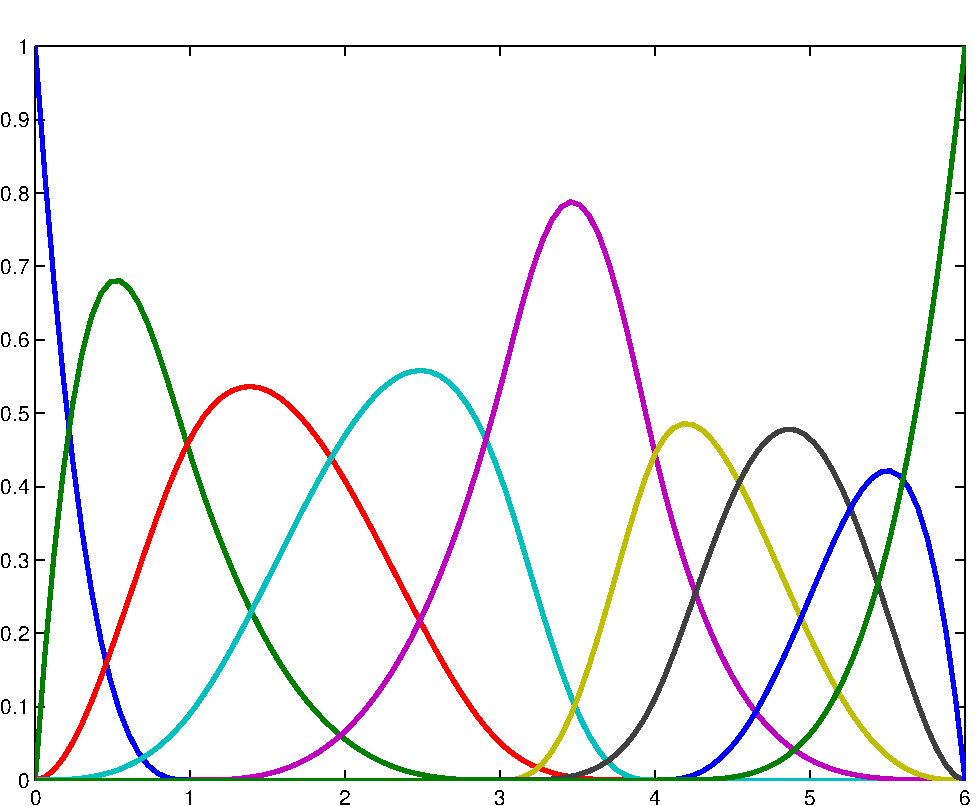
\includegraphics[width=4.5cm]{manual_ex_mdbspline0}
\end{center}

\smallskip
\noindent Now, do the same with periodic MDB-splines:
\medskip

\texttt{>> Hper = MDB\_extraction\_periodic(MP, rr, 2);}

\texttt{>> MDB\_visualization\_all(MP, Hper, 100, 'LineWidth', 2);}

\begin{center}
  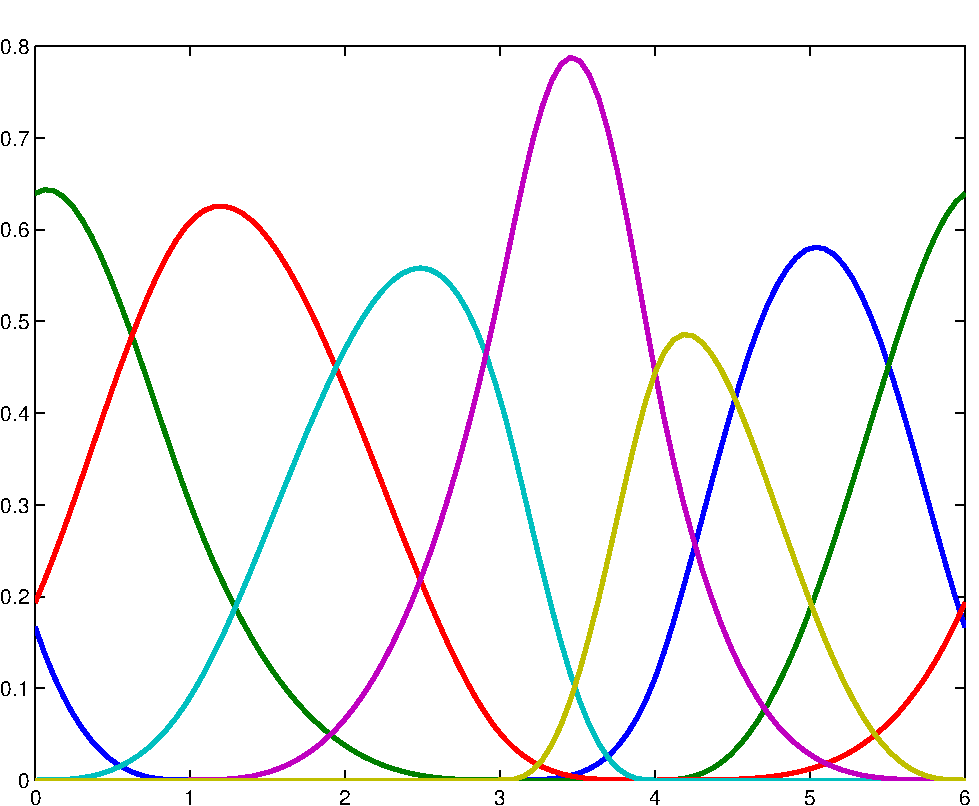
\includegraphics[width=4.5cm]{manual_ex_mdbspline0per}
\end{center}
\end{example}

%------------------------------------------------------------------

\subsubsection{MDB\_visualization\_spline} \label{sec:matlab-mdb-visualization-spline}

This function visualizes a spline in (periodic) MDB-spline form.

\syntax{MDB\_visualization\_spline(MP, H, cc, n, specs)}

\begin{inputlist}
  \paramitem{MP}{MDB-spline multi-patch}
  \paramitem{H}{extraction matrix}
  \paramitem{cc}{vector of coefficients}
  \paramitem{n}{number of evaluation points (optional)}
  \paramitem{specs}{pass any number of plot specifications (optional)}
\end{inputlist}

\begin{remark}
\noindent The extraction matrix \texttt{H} should be deduced from the MDB-spline multi-patch \texttt{MP} and incorporates the smoothness. 
Each element of the vector \texttt{cc} corresponds to an MDB-spline. Hence, \texttt{length(cc)} should be equal to \texttt{size(H,1)}.
The parameter \texttt{n} is a positive integer. When no value is specified, \texttt{n = 100} is assumed.
The parameter \texttt{specs} allows for any number of input arguments, which are passed on to the function \texttt{plot}. We refer the reader to the documentation of \texttt{plot} for all the plotting options.
\end{remark}

\begin{example}
\noindent Create an MDB-spline multi-patch with related smoothness vector and a vector of coefficients, and then plot the corresponding spline in MDB-spline form:
\medskip

\texttt{>> [MP, rr] = MDB\_patch\_poly([3, 3, 4, 4], [0, 1, 3, 4, 6], 2);}

\texttt{>> H = MDB\_extraction(MP, rr);}

\texttt{>> cc = [1, 2, 3, 4, 2, 2, 4, 3, 2];}

\texttt{>> MDB\_visualization\_spline(MP, H, cc, 100, 'LineWidth', 2);}

\begin{center}
  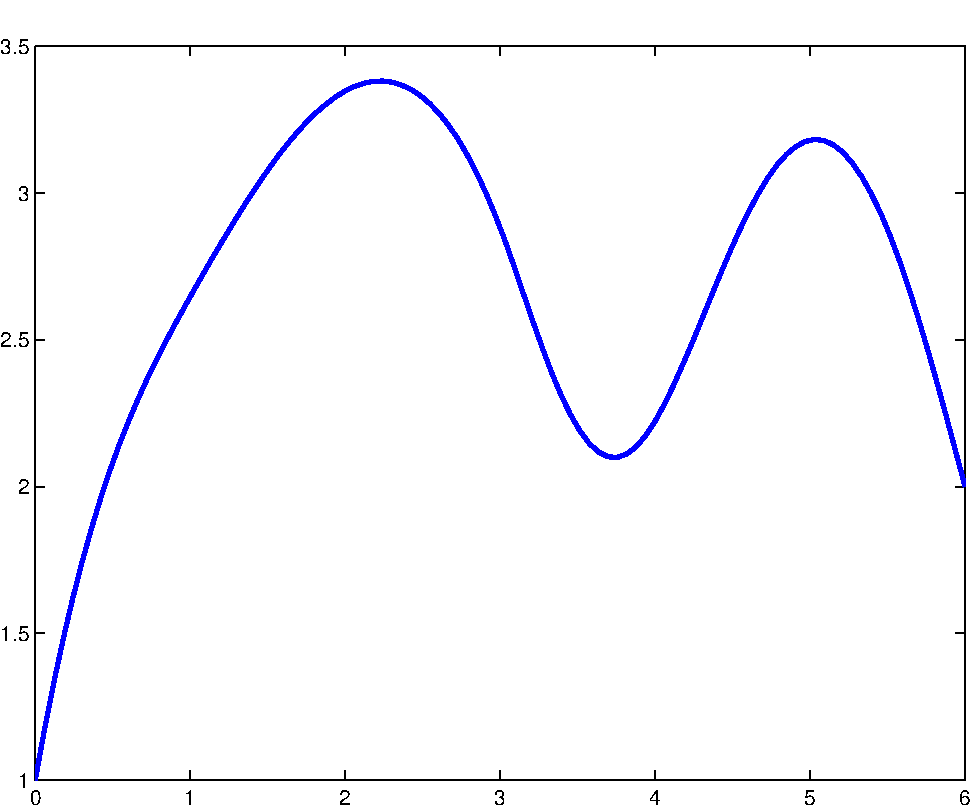
\includegraphics[width=4.5cm]{manual_ex_mdbspline1}
\end{center}
\vspace*{-0.35cm}
\end{example}

%------------------------------------------------------------------

\subsubsection{MDB\_conversion} \label{sec:matlab-mdb-conversion}

This function converts a spline in (periodic) MDB-spline form into another (periodic) MDB-spline form.
The conversion is exact when the source and destination MDB-spline multi-patches with smoothness imply nested spaces.

\pagebreak
\vspace*{-0.55cm}
\syntax{ccd = MDB\_conversion(MPd, Hd, MPs, Hs, ccs)}

\begin{inputlist}
  \paramitem{MPd}{destination MDB-spline multi-patch}
  \paramitem{Hd}{destination extraction matrix}
  \paramitem{MPs}{source MDB-spline multi-patch}
  \paramitem{Hs}{source extraction matrix}
  \paramitem{ccs}{source coefficient vector}
\end{inputlist}

\begin{outputlist}
  \paramitem{ccd}{destination coefficient vector}
\end{outputlist}

\begin{remark}
\noindent The MDB-spline multi-patches \texttt{MPs} and \texttt{MPd} must share the same number of B-spline patches, and preferably \texttt{MPd} contains also the same break points  as \texttt{MPs} for the best conversion results.
The extraction matrix \texttt{Hs} should be deduced from \texttt{MPs} and incorporates the smoothness. Similarly, the extraction matrix \texttt{Hd} should be deduced from \texttt{MPd} and incorporates the smoothness.
Each element of the vector \texttt{ccs} corresponds to an MDB-spline related to \texttt{Hs}. Hence, \texttt{length(ccs)} should be equal to \texttt{size(Hs,1)}. Similarly, each element of the resulting vector \texttt{ccd} corresponds to an MDB-spline related to \texttt{Hd}.
\end{remark}

\begin{example}
\noindent Create an MDB-spline multi-patch of multi-degree $(3,4)$ with related smoothness vector and a vector of coefficients; then, raise the multi-degree to $(5,7)$ and compute the coefficients of the new MDB-spline form:
\medskip

\texttt{>> [MPs, rrs] = MDB\_patch\_poly([3, 3, 4, 4], [0, 1, 3, 4, 6], 2);}

\texttt{>> Hs = MDB\_extraction(MPs, rrs);}

\texttt{>> ccs = [1, 2, 3, 4, 2, 2, 4, 3, 2];}

\texttt{>> [MPd, rrd] = MDB\_patch\_poly([5, 5, 7, 7], [0, 1, 3, 4, 6], 2);}

\texttt{>> Hd = MDB\_extraction(MPd, rrd);}

\texttt{>> ccd = MDB\_conversion(MPd, Hd, MPs, Hs, ccs)}

\texttt{ccd =}

\texttt{\ \ Columns 1 through 7}

\texttt{\ \ \ \ 1.0000\ \ \ \ 1.6000\ \ \ \ 2.0000\ \ \ \ 2.2646\ \ \ \ 2.8460\ \ \ \ 3.3714\ \ \ \ 3.5577}

\texttt{\ \ Columns 8 through 14}

\texttt{\ \ \ \ 3.4016\ \ \ \ 2.4308\ \ \ \ 2.2081\ \ \ \ 2.0673\ \ \ \ 2.0317\ \ \ \ 2.2222\ \ \ \ 2.9841}

\texttt{\ \ Columns 15 through 19}

\texttt{\ \ \ \ 3.3778\ \ \ \ 3.4476\ \ \ \ 3.1429\ \ \ \ 2.5714\ \ \ \ 2.0000}

%\medskip
\pagebreak
\noindent Now, keep the same multi-degree of the original spline but lower its smoothness, and compute the coefficients of the new MDB-spline form:
\medskip

\texttt{>> [MPe, rre] = MDB\_patch\_poly([3, 3, 4, 4], [0, 1, 3, 4, 6], 1);}

\texttt{>> He = MDB\_extraction(MPe, rre);}

\texttt{>> cce = MDB\_conversion(MPe, He, MPs, Hs, ccs)}

\texttt{cce =}

\texttt{\ \ Columns 1 through 7}

\texttt{\ \ \ \ 1.0000\ \ \ \ 2.0000\ \ \ \ 2.3333\ \ \ \ 3.2712\ \ \ \ 3.8136\ \ \ \ 2.5333\ \ \ \ 2.0000}

\texttt{\ \ Columns 8 through 12}

\texttt{\ \ \ \ 2.0000\ \ \ \ 2.6667\ \ \ \ 4.0000\ \ \ \ 3.0000\ \ \ \ 2.0000}

\medskip
\noindent Finally, find an approximation of the original spline using a lower multi-degree $(2,3)$:
\medskip

\texttt{>> [MPf, rrf] = MDB\_patch\_poly([2, 2, 2, 3, 3], [0, 1, 2, 3, 4, 6], 1);}

\texttt{>> Hf = MDB\_extraction(MPf, rrf);}

\texttt{>> ccf = MDB\_conversion(MPf, Hf, MPs, Hs, ccs)}

\texttt{ccf =}

\texttt{\ \ Columns 1 through 7}

\texttt{\ \ \ \ 1.0000\ \ \ \ 2.3034\ \ \ \ 3.1291\ \ \ \ 3.5633\ \ \ \ 2.3867\ \ \ \ 1.8105\ \ \ \ 3.1871}

\texttt{\ \ Columns 8 through 9}

\texttt{\ \ \ \ 3.7606\ \ \ \ 2.0000}
    
\medskip
\noindent Lowering the degree does not preserve the exact shape of the original spline, but it forms a reasonable approximation. Make a visual comparison between the original spline (blue) and the lower-degree spline (red):
\medskip

\texttt{>> MDB\_visualization\_spline(MPs, Hs, ccs, 50, 'LineWidth', 2, ...}

\texttt{>>\ \ \ \ \ \ \ \ \ \ \ \ \ 'Marker', 'o', 'MarkerSize', 10, 'Color', 'blue');}

\texttt{>> hold on;}

\texttt{>> MDB\_visualization\_spline(MPf, Hf, ccf, 50, 'LineWidth', 2, ...}

\texttt{>>\ \ \ \ \ \ \ \ \ \ \ \ \ 'Marker', '*', 'MarkerSize', 10, 'Color', 'red');}

\texttt{>> hold off;}

\begin{center}
  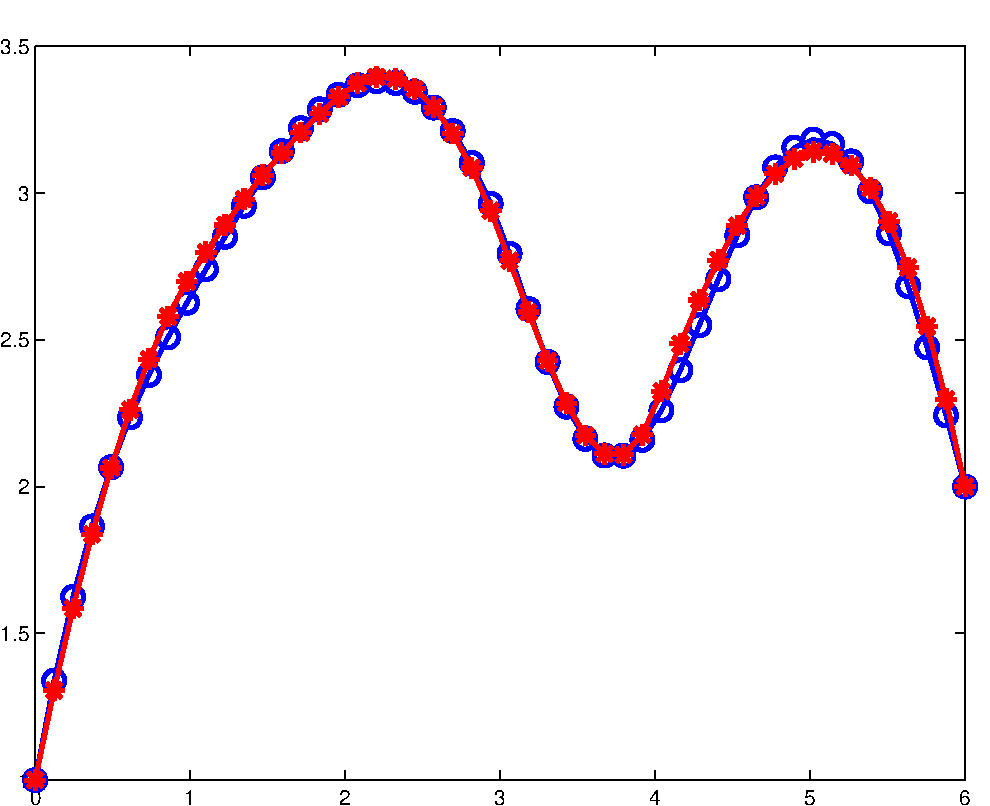
\includegraphics[width=4.5cm]{manual_ex_mdbspline2}
\end{center}
\end{example}


\end{document}
